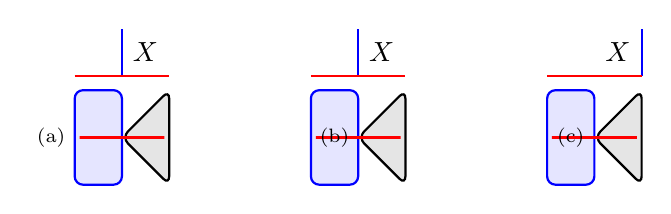
\begin{tikzpicture}[scale=0.6]
	\tikzset{every path/.style={thick,rounded corners=3pt}}
	\draw[blue,fill=blue!10] (-1,-1) -- (-1,1) -- (0,1) -- (0,-1) -- cycle;
	\draw[black,fill=black!10] (0,0) -- (1,-1) -- (1,1) -- cycle;
	\draw[red,fill=red!10] (-1,0) -- (0,0) -- (1,0) -- cycle;
	\draw[blue,fill=blue!10] (4,-1) -- (4,1) -- (5,1) -- (5,-1) -- cycle;
	\draw[black,fill=black!10] (5,0) -- (6,-1) -- (6,1) -- cycle;
	\draw[red,fill=red!10] (4,0) -- (5,0) -- (6,0) -- cycle;
	\draw[blue,fill=blue!10] (9,-1) -- (9,1) -- (10,1) -- (10,-1) -- cycle;
	\draw[black,fill=black!10] (10,0) -- (11,-1) -- (11,1) -- cycle;
	\draw[red,fill=red!10] (9,0) -- (10,0) -- (11,0) -- cycle;
	\draw[blue,fill=blue!10] (0,1.3) -- (0,2.3);
	\draw[red,fill=red!10] (-1,1.3) -- (0,1.3) -- (1,1.3);
	\draw[blue,fill=blue!10] (5,1.3) -- (5,2.3);
	\draw[red,fill=red!10] (4,1.3) -- (5,1.3) -- (6,1.3);
	\draw[blue,fill=blue!10] (11,1.3) -- (11,2.3);
	\draw[red,fill=red!10] (9,1.3) -- (10,1.3) -- (11,1.3);
	\node at (-1.5,0) {\scriptsize{(a)}};
	\node at (4.5,0) {\scriptsize{(b)}};
	\node at (9.5,0) {\scriptsize{(c)}};
	\node at (0.5,1.8) {$X$};
	\node at (5.5,1.8) {$X$};
	\node at (10.5,1.8) {$X$};
\end{tikzpicture}